\documentclass[sigconf]{acmart}
\usepackage{tikz}
\usetikzlibrary{shapes.geometric}
\usetikzlibrary{matrix}
\usetikzlibrary{graphs}
\usetikzlibrary{shapes.geometric}
\usepackage{pgfplots}
\pgfplotsset{compat=1.18} % Recommended for modern TikZ/pgfplots
\usepackage{environ}
\usepackage{ifthen}
%%
%% \BibTeX command to typeset BibTeX logo in the docs
\AtBeginDocument{%
  \providecommand\BibTeX{{%
    Bib\TeX}}}

\setcopyright{acmlicensed}
\copyrightyear{2025}
\acmYear{2025}
\acmDOI{XXXXXXX.XXXXXXX}
%% These commands are for a PROCEEDINGS abstract or paper.
\acmConference[FPGA '26]{International Symposium on Field Programable Gate Arrays}{June 03--05,
  2025}{Seaside, CA}
%%
%%  Uncomment \acmBooktitle if the title of the proceedings is different
%%  from ``Proceedings of ...''!
%%
%%\acmBooktitle{Woodstock '18: ACM Symposium on Neural Gaze Detection,
%%  June 03--05, 2018, Woodstock, NY}
\acmISBN{978-1-4503-XXXX-X/2018/06}

\begin{document}

\title{Yet Another Multi-Port Memory for FPGAs Using XOR and LVT Methods}

%%
%% The "author" command and its associated commands are used to define
%% the authors and their affiliations.
%% Of note is the shared affiliation of the first two authors, and the
%% "authornote" and "authornotemark" commands
%% used to denote shared contribution to the research.
%\author{Kevin Townsend}
\author{XXX}
\email{XXX@XXX}

%\renewcommand{\shortauthors}{Townsend}
\renewcommand{\shortauthors}{XXX}

\begin{abstract}
  We propose a simple extention to XOR memories presented in previous work.
In this paper we generalize the XOR memory allowing for any number of full, read-only and write-only ports.
FPGAs.This paper also presents a novel and efficient architecture for creating live value table memory using an XOR-based scheme, emphasizing its bidirectional capabilities.

This is achieved by exploiting the properties of XOR, allowing any data entry to be reconstructed by XORing the corresponding entries from all memory banks. The result is a high-throughput, coherent multi-ported memory that is particularly well-suited for implementation on FPGAs.

We use an XOR memory with full ports to implement a live value table (LVT) design.
We evaluate the architecture's performance and resource utilization, showing that it uses significantly less logic and can achieve higher frequencies for deep memory configurations compared to LVT-based designs. This makes the XOR-based bidirectional live value table a compelling alternative for applications requiring high-performance, flexible memory access.
\end{abstract}

%%
%% The code below is generated by the tool at http://dl.acm.org/ccs.cfm.
%% Please copy and paste the code instead of the example below.
%%
%\begin{CCSXML}
%<ccs2012>
% <concept>
%  <concept_id>00000000.0000000.0000000</concept_id>
%  <concept_desc>Do Not Use This Code, Generate the Correct Terms for Your Paper</concept_desc>
%  <concept_significance>500</concept_significance>
% </concept>
% <concept>
%  <concept_id>00000000.00000000.00000000</concept_id>
%  <concept_desc>Do Not Use This Code, Generate the Correct Terms for Your Paper</concept_desc>
%  <concept_significance>300</concept_significance>
% </concept>
% <concept>
%  <concept_id>00000000.00000000.00000000</concept_id>
%  <concept_desc>Do Not Use This Code, Generate the Correct Terms for Your Paper</concept_desc>
%  <concept_significance>100</concept_significance>
% </concept>
% <concept>
%  <concept_id>00000000.00000000.00000000</concept_id>
%  <concept_desc>Do Not Use This Code, Generate the Correct Terms for Your Paper</concept_desc>
%  <concept_significance>100</concept_significance>
% </concept>
%</ccs2012>
%\end{CCSXML}
%
%\ccsdesc[500]{Do Not Use This Code~Generate the Correct Terms for Your Paper}
%\ccsdesc[300]{Do Not Use This Code~Generate the Correct Terms for Your Paper}
%\ccsdesc{Do Not Use This Code~Generate the Correct Terms for Your Paper}
%\ccsdesc[100]{Do Not Use This Code~Generate the Correct Terms for Your Paper}

%%
%% Keywords. The author(s) should pick words that accurately describe
%% the work being presented. Separate the keywords with commas.
%\keywords{Do, Not, Us, This, Code, Put, the, Correct, Terms, for,
%  Your, Paper}
%% A "teaser" image appears between the author and affiliation
%% information and the body of the document, and typically spans the
%% page.
\begin{teaserfigure}
  %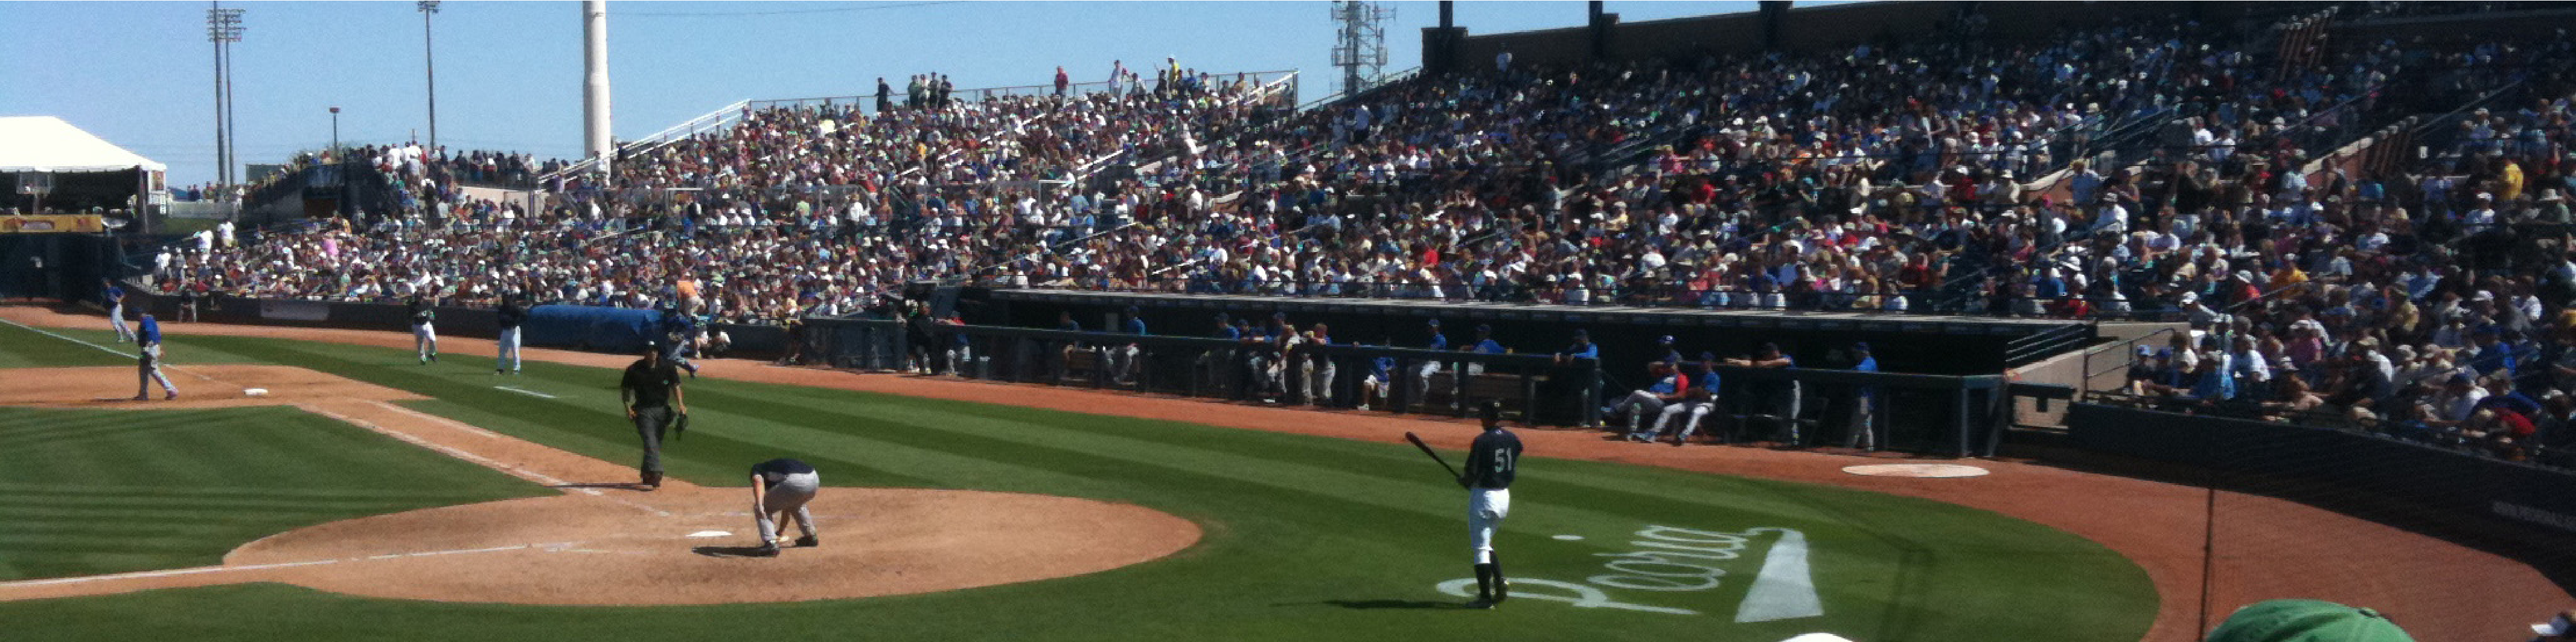
\includegraphics[width=\textwidth]{sampleteaser}
  \begin{center}
  %\begin{scaletikzpicturetowidth}{\textwidth}
  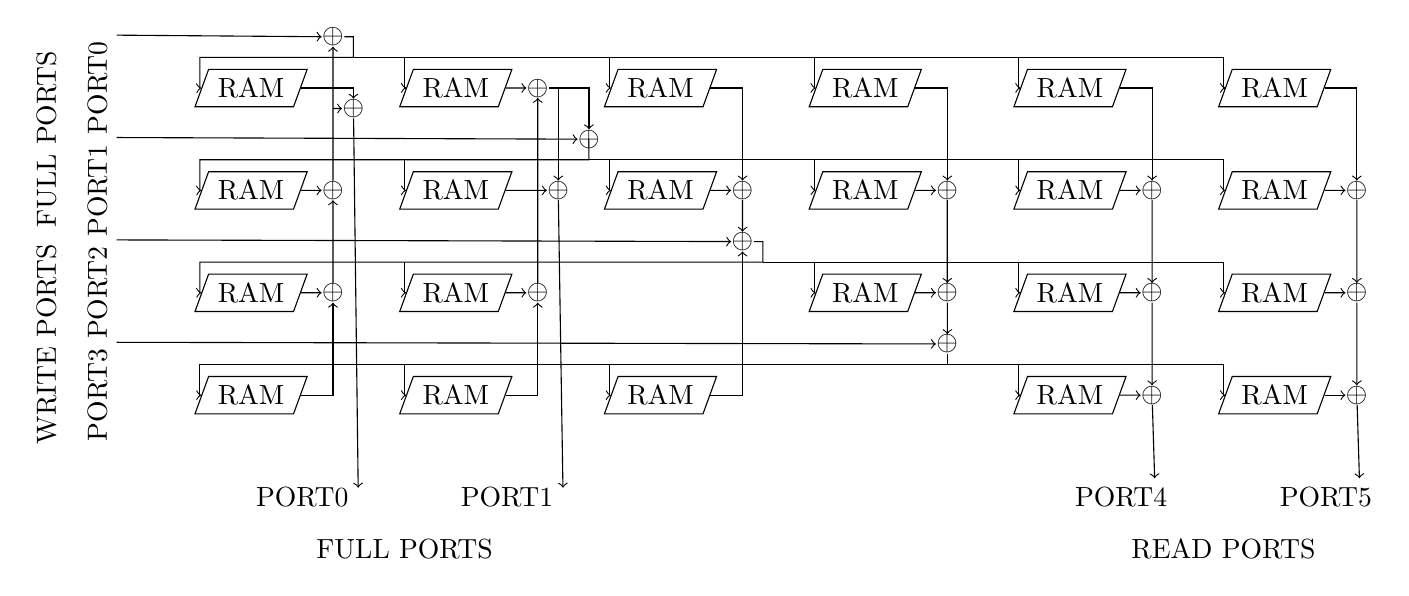
\begin{tikzpicture}[scale=1.3]
  \foreach \x in {0,1,2,3,4,5} {
    \foreach \y in {0,1,2,3} {
      \ifthenelse{\(\x = 2 \AND \y = 1\) \OR \(\x = 3 \AND \y = 0\)}{}{
        \node (r\x\y)[trapezium, trapezium left angle=70, trapezium right angle=110, draw] at (2*\x, \y){RAM};
      }
    }
  }
  \foreach \x in {0,1,4,5} {
    \node (bport\x)[] at (2*\x+.5, -1){PORT\x};
  }
  \foreach \y in {0,1,2,3} {
    \node (lport\y)[rotate=90] at (-1.5, 3-\y){PORT\y};
  }
  \node [rotate=90] at (-2, .5){WRITE PORTS};
  \node [rotate=90] at (-2, 2.5){FULL PORTS};
  \node [] at (1.5, -1.5){FULL PORTS};
  \node [] at (9.5, -1.5){READ PORTS};
  \node(x50)[inner sep=0pt] at (10.8, 0){$\oplus$};
  \node(x51)[inner sep=0pt] at (10.8, 1){$\oplus$};
  \node(x52)[inner sep=0pt] at (10.8, 2){$\oplus$};
  \draw[->] (r50) -- (x50);
  \draw[->] (r51) -- (x51);
  \draw[->] (r52) -- (x52);
  \draw[->] (r53) -| (x52);
  \draw[->] (x52) -- (x51);
  \draw[->] (x51) -- (x50);
  \draw[->] (x50) -- (bport5.30);
  \node(x40)[inner sep=0pt] at (8.8, 0){$\oplus$};
  \node(x41)[inner sep=0pt] at (8.8, 1){$\oplus$};
  \node(x42)[inner sep=0pt] at (8.8, 2){$\oplus$};
  \draw[->] (r40) -- (x40);
  \draw[->] (r41) -- (x41);
  \draw[->] (r42) -- (x42);
  \draw[->] (r43) -| (x42);
  \draw[->] (x42) -- (x41);
  \draw[->] (x41) -- (x40);
  \draw[->] (x40) -- (bport4.30);
  \node(x31)[inner sep=0pt] at (6.8, 1){$\oplus$};
  \node(x32)[inner sep=0pt] at (6.8, 2){$\oplus$};
  \node(x30)[inner sep=0pt] at (6.8, .5){$\oplus$};
  \draw[->] (r31) -- (x31);
  \draw[->] (r32) -- (x32);
  \draw[->] (r33) -| (x32);
  \draw[->] (x32) -- (x31);
  \draw[->] (x31) -- (x30);
  %PORT3 connections.
  \draw[->] (lport3.340) -- (x30);
  \draw[->] (x30) |- (-.5,.3) |- (r00);
  \draw[->] (1.5,.3) |- (r10);
  \draw[->] (3.5,.3) |- (r20);
  \draw[->] (6.8, .3) -| (7.5,0) -- (r40);
  \draw[->] (7.5, .3) -| (9.5,0) -- (r50);
  %PORT2 XORs
  \node(x22)[inner sep=0pt] at (4.8, 2){$\oplus$};
  \node(x21)[inner sep=0pt] at (4.8, 1.5){$\oplus$};
  %PORT2 connections
  \draw[->] (lport2.340) -- (x21);
  \draw[->] (r23) -| (x22);
  \draw[->] (r22) -- (x22);
  \draw[->] (x22) -- (x21);
  \draw[->] (r20) -| (x21);
  \draw[->] (x21) -| (5,1.3) -| (-.5,1) -- (r01);
  \draw[->] (1.5,1.3) |- (r11);
  \draw[->] (5,1.3) -- (9.5, 1.3) |- (r51);
  \draw[->] (7.5, 1.3) |- (r41);
  \draw[->] (5.5, 1.3) |- (r31);
  %draw xor of full ports
  %PORT1
  \node(x11)[inner sep=0pt] at (2.8, 1){$\oplus$};
  \node(x12)[inner sep=0pt] at (3.3, 2.5){$\oplus$};
  \node(x12b)[inner sep=0pt] at (3, 2){$\oplus$};
  \node(x13)[inner sep=0pt] at (2.8, 3){$\oplus$};
  \draw[->] (r10) -| (x11);
  \draw[->] (r11) -- (x11);
  \draw[->] (lport1.340) -- (x12);
  \draw[->] (x11) -- (x13);
  \draw[->] (r13) -- (x13);
  \draw[->] (x13) -| (x12);
  \draw[->] (r12) -- (x12b);
  \draw[->] (x12) -| (3.3, 2.3) -| (-.5,2) -- (r02);
  \draw[->] (1.5,2.3) |- (r12);
  \draw[->] (3.3, 2.3) -- (9.5, 2.3) |- (r52);
  \draw[->] (3.5, 2.3) |- (r22);
  \draw[->] (5.5, 2.3) |- (r32);
  \draw[->] (7.5, 2.3) |- (r42);
  \draw[->] (x13) -| (x12b);
  \draw[->] (x12b) -- (bport1.10);
  %PORT0
  \node(x01)[inner sep=0pt] at (0.8, 1){$\oplus$};
  \node(x02)[inner sep=0pt] at (0.8, 2){$\oplus$};
  \node(x03)[inner sep=0pt] at (0.8, 3.5){$\oplus$};
  \node(x03b)[inner sep=0pt] at (1.0, 2.8){$\oplus$};
  \draw[->] (r00) -| (x01);
  \draw[->] (r01) -- (x01);
  \draw[->] (x01) -- (x02);
  \draw[->] (x02) -- (x03);
  \draw[->] (lport0.340) -- (x03);
  \draw[->] (x03) -| (1, 3.3) -| (-.5,3) -- (r03);
  \draw[->] (1, 3.3) -- (9.5, 3.3) |- (r53);
  \draw[->] (1.5, 3.3) |- (r13);
  \draw[->] (3.5, 3.3) |- (r23);
  \draw[->] (5.5, 3.3) |- (r33);
  \draw[->] (7.5, 3.3) |- (r43);
  \draw[->] (.8, 2.8) -- (x03b);
  \draw[->] (r02) -- (x02);
  \draw[->] (r03) -| (x03b);
  \draw[->] (x03b) -- (bport0.10);
  \end{tikzpicture}
  %\end{scaletikzpicturetowidth}
  \end{center}
  \caption{A multi-port memory with 2 full ports, 2 write-only ports and 2 read-only ports.}
  \Description{Enjoying the baseball game from the third-base
  seats. Ichiro Suzuki preparing to bat.}
  \label{fig:teaser}
\end{teaserfigure}

\received{20 February 2007}
\received[revised]{12 March 2009}
\received[accepted]{5 June 2009}

%%
%% This command processes the author and affiliation and title
%% information and builds the first part of the formatted document.
\maketitle

\section{Motivation}

As computation needs keep increasing, one way to keep up with Moore's Law has been
specialized architectures. FPGAs provide a way to implement architectures without taping out an ASIC.
However, the limitations of FPGA resources means some creativity is needed to map designs to FPGAs.
This paper explores the limitation of FPGAs in the fact that FPGA memories have a limited number of
ports. Specifically we look at creating memories with more than 2 ports.

The 3 major FPGA vendors\cite{amd20,intel24,lattice21} implement distributed memory (small memories) and block memory (large memories)
differently, however they share some characteristics.

All 3 vendors support distributed memory configurations with 1 full port and between 1 to 3 read ports.

All 3 vendors support block memory with 2 full ports. None of the vendors support memories with more than 2 full ports.

Although this limitation is problematic for designs requiring multiple ports particularly write or full ports, we show that these resources make it possible to achieve high throughput quad and octal full port memories.

\section{Source Code}
We provide all of the source code used in implementation and testing our design at
https://anonymous.4open.science/r/mpm-7666/. We tested our design with Verilator and implemented the design
with Vivado (Xilinx/AMD).

\section{XOR memory}

We propose a simple generalization to XOR memories presented in previous work\cite{laforest14}.
XOR memories work by using the $a \oplus b \oplus b = a$ property. We add bidirectional
ports and analyze the perforamance of distributed memory and block memory
versions of this design. We also present applications for these memories.

The number of RAMs needed is: $(W+F)(W+F+R)-W$, which expands to: $W^2 + 2WF + F^2 + WR + FR - W$.

Reading data from an XOR memory simply involves XORing all of the data from the RAMs in one column from the same address. For example say address $x$ has values $A$, $B$, $C$ and $D$, the data read would be $A\oplus B\oplus C \oplus D$.

Writing to the memory involves reading from all memories except the current row (say row/port 2 in the example) and XORing the incoming data $E$ (in the example this results in $A\oplus B \oplus D \oplus E$) and storing that value in all the RAMs in that row.

The next time that data is read the result will be $A\oplus B \oplus (A \oplus B\oplus D\oplus E) \oplus D$, which equals $E$.

You may notice that writing to a port involves XORing all but one stored value and reading involves XORing all values. This enables full ports to be created just by adding one RAM to what would otherwise be just a write port.

Note that this memory requires that all of the RAMs in a row have the same data. Initializing the rams to the same data (e.g. all 0s) is required for the memory to operate properly. This is not an issue in FPGAs since the memory can be initialized to 0. since rows are written to at the same time as long as the memories are intially the same they will remain the same.

\section{Live Value Table Memory}
\begin{figure}
  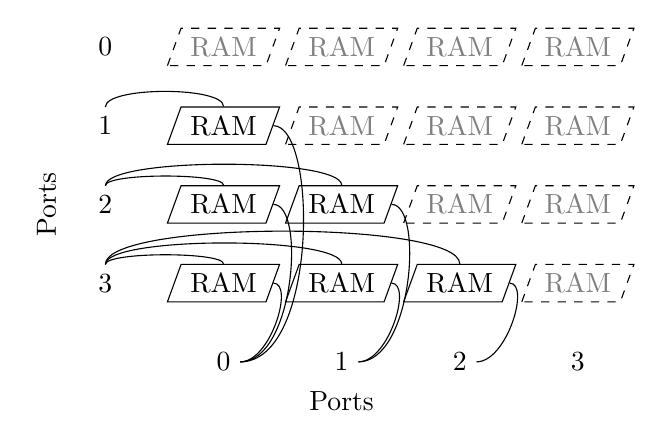
\begin{tikzpicture}[xscale=1.5]
  %draw rams
  \foreach \x in {0,1,2,3} {
    \foreach \y in {0,1,2,3} {
      \ifthenelse{\x < \y}{
      \node(r\y\x)[trapezium, trapezium left angle=70, trapezium right angle=110, draw] at (\x,3-\y) {RAM};
      }{
      \node[text=gray,dashed, trapezium, trapezium left angle=70, trapezium right angle=110, draw] at (\x,3-\y) {RAM};
      }
    }
  }
  %draw a ports
  \foreach \x in {0,1,2,3} {
    \node(xport\x) at (\x, -1) {\x};
  }
  %draw b ports
  \foreach \y in {0,1,2,3} {
    \node(yport\y) at (-1, 3-\y) {\y};
  }
  %draw connections
  %x0 connections
  \draw (xport0) .. controls (.8,-1) and (.8,2) .. (r10.east);
  \draw (xport0) .. controls (.6,-1) and (.7,1) .. (r20.east);
  \draw (xport0) .. controls (.4,-1) and (.6,0) .. (r30.east);
  %x1 connections
  \draw (xport1) .. controls (1.6,-1) and (1.7,1) .. (r21);
  \draw (xport1) .. controls (1.4,-1) and (1.6,0) .. (r31);
  %x2 connection
  \draw (xport2) .. controls (2.4,-1) and (2.6,0) .. (r32);
  %y1 connection
  \draw (yport1) .. controls (-1, 2.5) and (0, 2.5) .. (r10);
  %y2 connections
  \draw (yport2) .. controls (-1, 1.4) and (0, 1.4) .. (r20);
  \draw (yport2) .. controls (-1, 1.6) and (1, 1.6) .. (r21);
  %y3 connections
  \draw (yport3) .. controls (-1, 0.4) and (0, 0.4) .. (r30);
  \draw (yport3) .. controls (-1, 0.6) and (1, 0.6) .. (r31);
  \draw (yport3) .. controls (-1, 0.8) and (2, 0.8) .. (r32);
  %draw labels
  \node at (-1.5, 1)[rotate=90]{Ports};
  \node at (1, -1.5){Ports};
  \end{tikzpicture}
  \caption{Multiport memory created with dual-port memories.}
  \Description{An illustration.}
\end{figure}

\begin{figure}
  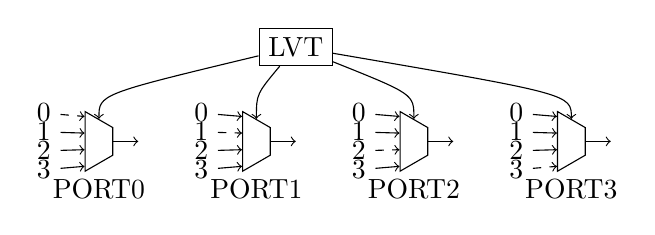
\begin{tikzpicture}[yscale=1.2]
    \node(lvt)[draw] at (2.5, 1) {LVT};
    \foreach \x in {0,1,2,3}{
    \node(mux\x)[draw,trapezium, rotate=-90,inner sep=5pt] at (2*\x,0){};
    \node(mux\x port0) at (2*\x-.7,.3){0};
    \node(mux\x port1) at (2*\x-.7,.1){1};
    \node(mux\x port2) at (2*\x-.7,-.1){2};
    \node(mux\x port3) at (2*\x-.7,-.3){3};
    \ifthenelse{\x=0}{
    \draw[->,dashed] (mux\x port0) -- (mux\x.210);
    }{
    \draw[->] (mux\x port0) -- (mux\x.210);
    }
    \ifthenelse{\x=1}{
    \draw[->,dashed] (mux\x port1) -- (mux\x.240);
    }{
    \draw[->] (mux\x port1) -- (mux\x.240);
    }
    \ifthenelse{\x=2}{
    \draw[->,dashed] (mux\x port2) -- (mux\x.300);
    }{
    \draw[->] (mux\x port2) -- (mux\x.300);
    }
    \ifthenelse{\x=3}{
    \draw[->,dashed] (mux\x port3) -- (mux\x.330);
    }{
    \draw[->] (mux\x port3) -- (mux\x.330);
    }
    \draw[->] (mux\x ) -- (2*\x+.5,0);
    \node at (2*\x,-.5) {PORT\x};
    }
    \draw[->] (lvt) .. controls (0,.5) .. (mux0);
    \draw[->] (lvt) .. controls (2,.5) .. (mux1);
    \draw[->] (lvt) .. controls (4,.5) .. (mux2);
    \draw[->] (lvt) .. controls (6,.5) .. (mux3);
  \end{tikzpicture}
  \caption{LVT Multiport memory created with dual-port memories.}
  \Description{An illustration.}
\end{figure}

XOR memories can be used by themselves, however a live value table (LVT) may be more efficient.

We present a LVT memory that utilises distrubuted memory xor live value table.

In \cite{laforest12} the live value table was implemented with registers. Previous work used
distributed memory \cite{abdelhadi16}. However they did not use bidirectional xor ports in their implementation.

We create a LVT memory using the technique described in \cite{choi12}. This live value memory is composed of 2-(full)port memories. Each port shares a RAM with another port. This results in $N(N-1)/2$ RAMs being needed. See figure (todo cite figure).

The memory gets its name because of a multiport memory that tracks the most recent stored value (aka a live value table). The point of a multi-port memory that requires a multi-port memory is that wide (e.g. 32 bit data) can be stored more effeciently this way.

Instead of using a register based live-value table as in \cite{choi12} we use a xor memory similar to \cite{abdelhadi16}.

We show we utilize x\% less resources than LVT and I-LVT.

\section{Implementation}

We explore designs with 4 to 32 ports. Although 16 and 32 port designs fit on large FPGAs, we believe smaller 4 and 8 port designs are more practical. We say
more practical because of the high resource usage of XOR and LVT memories at high port counts.
N**2 for XOR and N*(N-1)/2 for LVT. However we were able to synthesize a 32 port memory.

Without write delay an 8 port memory runs at Xmhz (x\% of max). With write delay and pipelining the design runs at Xmhz (x\% of max).

\begin{figure}
  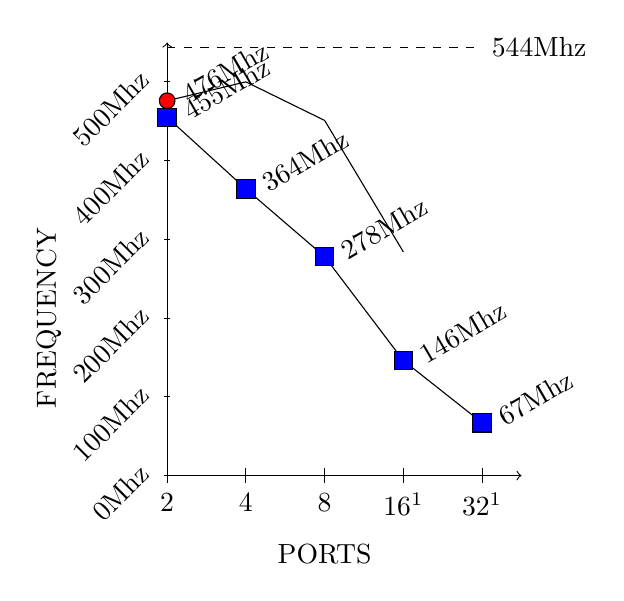
\begin{tikzpicture}
    \draw[->] (0,0) -- (4.5, 0);
    \draw (0,.1) -- (0, -.1) node[anchor=north] {2};
    \draw (1,.1) -- (1, -.1) node[anchor=north] {4};
    \draw (2,.1) -- (2, -.1) node[anchor=north] {8};
    \draw (3,.1) -- (3, -.1) node[anchor=north] {16\footnotemark[1]};
    \draw (4,.1) -- (4, -.1) node[anchor=north] {32\footnotemark[1]};
    %draw y axis
    \draw[->] (0,0) -- (0, 5.5);
    \draw (1pt, 0) -- (-1pt, 0) node[rotate=45,anchor=south east] {0Mhz};
    \foreach \y in {1,2,3,4,5}
      \draw (1pt, \y) -- (-1pt, \y) node[rotate=45,anchor=south east] {\y00Mhz};
    %labels
    \node at (2,-1) {PORTS};
    \node at (-1.5,2) [rotate=90]{FREQUENCY};
    %max frequncy
    \draw[dashed] (0, 5.44) -- (4, 5.44) node[anchor=west] {544Mhz};
    %line graphs
    \draw (0, 4.55) -- (1, 3.64) -- (2, 2.78) -- (3, 1.46) -- (4, 0.67);
    \node[fill=blue, draw,label={[rotate=30]right:455Mhz}] at (0,4.55){};
    \node[fill=blue, draw,label={[rotate=30]right:364Mhz}] at (1,3.64){};
    \node[fill=blue, draw,label={[rotate=30]right:278Mhz}] at (2,2.78){};
    \node[fill=blue, draw,label={[rotate=30]right:146Mhz}] at (3,1.46){};
    \node[fill=blue, draw,label={[rotate=30]right:67Mhz}] at (4,.67){};
    %line graph for pipelnined.
    \draw (0, 4.76) -- (1, 5.00) -- (2, 4.51) -- (3, 2.84);
    \node[fill=red, draw, circle,inner sep=2pt,label={[rotate=30]right:476Mhz}] at (0,4.76){};
  \end{tikzpicture}
  \caption{Frequency of design.}
  \Description{A graph showing the frequency of the design for difference port counts.}
\end{figure}

\footnotetext{To reduce the number of IO ports and fit the design on the FPGA we used a wrapper for the multi-port memory for designs with 16 and 32 ports.}

\begin{table}
  \caption{Synthesis results for different port counts}
  \label{tab:syn}
  \begin{tabular}{lllll}
    \toprule
    Ports & LUTS & FF & BRAM & Max Frequency\\
    \midrule
    2 & 127 & 0 & 1 & 455Mhz\\
    4 & 640 & 0 & 6 & 364Mhz\\
    8 & 3,012 & 0 & 28 & 278Mhz\\
    16\footnotemark[1] & 16,544 & 0 & 120 & 146Mhz\\
    32\footnotemark[1] & 85,728 & 0 & 496 & 67Mhz\\
    \bottomrule
  \end{tabular}
\end{table}

\begin{table}
  \caption{Synthesis results for different port counts for pipelined design}
  \label{tab:synpiped}
  \begin{tabular}{lllll}
    \toprule
    Ports & LUTS & FF & BRAM & Max Frequency\\
    \midrule
    2 & 111 & 26 & 1 & 476Mhz\\
    4 & 708 & 64 & 6 & 500Mhz\\
    8 & 3,092 & 152 & 28 & 451Mhz\\
    16\footnotemark[1] & 16,800 & 448 & 120 & 284Mhz\\
    32\footnotemark[1] & 86,608 & 1,502 & 496 & XMhz\\
    \bottomrule
  \end{tabular}
\end{table}
\section{Conclusion}
Several solutions to the port limit on FPGAs other than what is presented here.
For example multi-pumping and banking. multi-pumping is the process of reducing
the clock speed to increase the number of ports. For example a 300Mhz single
port memory can handle 2 150Mhz ports. Banking requires stalls and routing logic
due to the segmented memory. Our design uses replication and some creativity
XOR and LVT to create multiple ports.

%% The next two lines define the bibliography style to be used, and
%% the bibliography file.
\bibliographystyle{ACM-Reference-Format}
\bibliography{paper}


%%
%% If your work has an appendix, this is the place to put it.
%\appendix

\end{document}
\endinput
%%
%% End of file `sample-sigconf.tex'.
